Elliptic curves and bla and bla and bla. See
\cite{silverman:elliptic,silverman:advanced,blake+seroussi+smart}.

\section{Definitions}
\label{sec:definitions}

We let $\K$ be a field and $\clot{\K}$ be its algebraic
closure. \index{elliptic~curve}Elliptic curves are genus $1$ curves
over $\clot{\K}$ with a distinguished point.

\subsection{Weierstrass equations}
\label{sec:weierstr-equat}

\begin{definition}[Weierstrass equation]
  \index{Weierstrass~equation} Any elliptic curve $E$ can be viewed as
  the projective variety associated to the equation
  \begin{equation}
    \label{eq:107}
    E\;:\; Y^2Z + a_1XYZ + a_3YZ^2 = X^3 + a_2X^2Z + a_4XZ^2 + a_6Z^3
    \text{,}
  \end{equation}
  with $a_1,\ldots,a_6\in\clot{\K}$.  The distinguished point is
  $[0:1:0]$, called the \index{point~at~infinity}\emph{point at
    infinity} and denoted by $\0$\nomenclature[O]{$\0$}{Point at
    infinity of an elliptic curve}.  When $a_1,\ldots,a_6\in\K$, the
  curve is said to be \emph{defined over $\K$}.
\end{definition}

Eq.~\eqref{eq:107} is called the \emph{homogeneous Weierstrass
  form}\index{Weierstrass~form!homogeneous} of the curve $E$.  After
the change of variables $x=\frac{X}{Z},y=\frac{Y}{Z}$,
Eq.~\eqref{eq:107} can be rewritten as
\begin{equation}
  \label{eq:112}
  E\;:\;y^2 + a_1xy + a_3y = x^3 + a_2x^2 + a_4x + a_6
  \text{,}
\end{equation}
called the \emph{affine Weierstrass
  form}\index{Weierstrass~form!affine}. Then the curve $E$ is the
locus of zeros of Eq.~\eqref{eq:112} in $\clot{\K}^2$ (or, more
exactly, in the affine plane $\mathbb{A}^2$), plus the extra point at
infinity $\0$.

\begin{definition}[Function field]
  If $E$ is an elliptic curve defined by an affine Weierstrass
  equation $f(x,y)=0$ with coefficients in $\K$, we denote by $\K(E)$%
  \nomenclature[KE]{$\K(E)$}{Function field of an elliptic curve} the
  field of fractions of
  \begin{equation}
    \label{eq:125}
    K[E]=K[x,y]/(f(x,y))
    \text{,}
  \end{equation}
  and call it the \index{function~field}\emph{function field} of $E$
  over $\K$.
\end{definition}

The \index{discriminant~of~an~elliptic~curve}discriminant of
Eq.~\eqref{eq:112} is
\begin{equation}
  \label{eq:118}
  \Delta_E = -b_2^2b_8-8b_4^3-27b_6^2+9b_2b_4b_6
  \text{,}
\end{equation}
where
\begin{equation}
  \label{eq:117}
  \begin{aligned}
    b_2 &= a_1^2 + 4a_2\text{,}\\
    b_4 &= 2a_4 + a_1a_3\text{,}\\
    b_6 &= a_3^2 + 4a_6\text{,}\\
    b_8 &= a_1^2a_6+4a_2a_6-a_1a_3a_4+a_2a_3^2-a_4^2\text{.}
  \end{aligned}
\end{equation}

\begin{remark}
  The curve defined by~\eqref{eq:112} has an unique singular point if
  and only if $\Delta_E=0$.  Figure~\ref{fig:singular} shows the two
  possible shapes of a singular curve over the reals. Then, every line
  passing through the singular point meets the curve in another unique
  point. This parameterization makes $E$ birationally equivalent to
  $\Proj^1$, thus $E$ has genus $0$. The converse is also true, thus
  Eq.~\eqref{eq:112} defines an elliptic curve if and only if
  $\Delta_E\ne0$.
\end{remark}


\begin{figure}[ht]
  \centering
  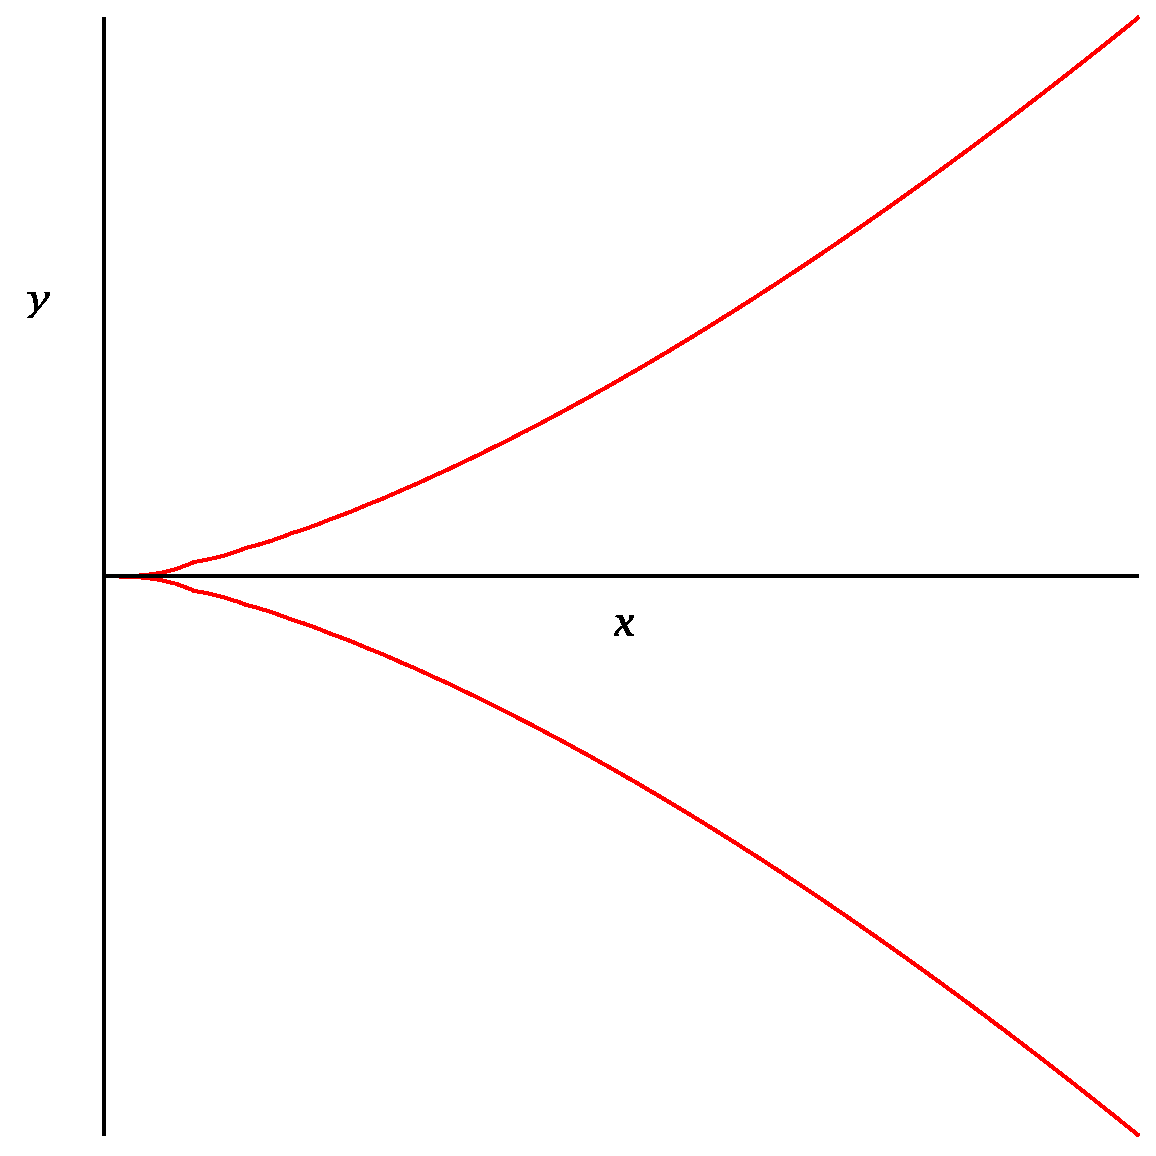
\includegraphics[width=0.45\textwidth]{isogeny/cusp}
  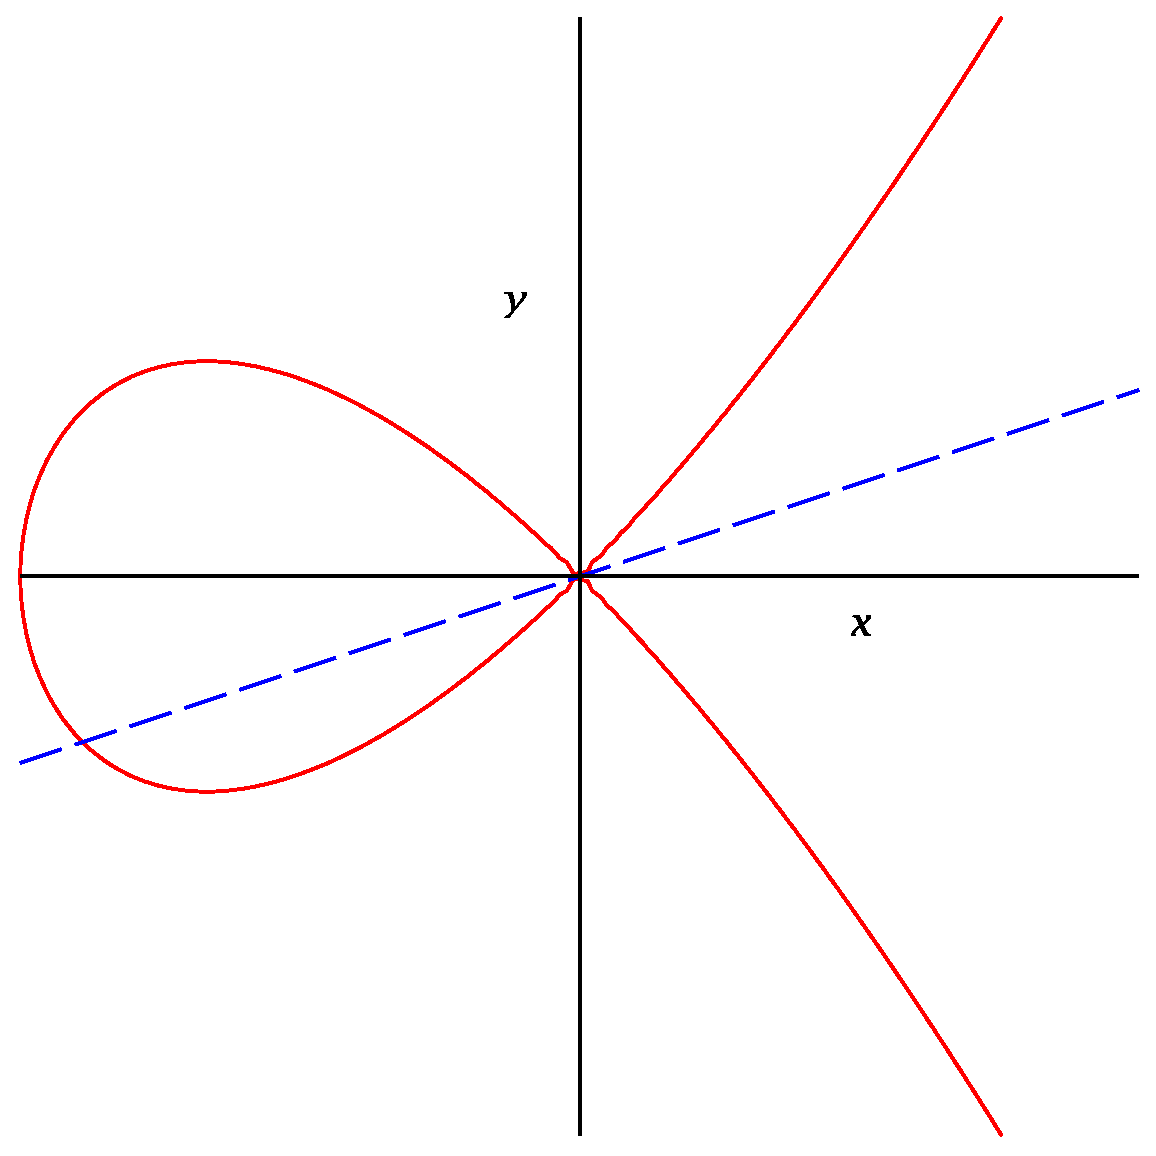
\includegraphics[width=0.45\textwidth]{isogeny/node}
  \caption{Two singular Weierstrass curves. On the left $y^2=x^3$, on
    the right $y^2=x^3+x^2$. On the right we have shown the
    parameterization by the line passing through the origin.}
  \label{fig:singular}
\end{figure}

\begin{definition}[$j$-invariant]
  \index{j-invariant@$j$-invariant}%
  \nomenclature[j]{$j_E$}{$j$-invariant of an elliptic curve $E$}
  We associate to the curve $E$ defined by Eq.~\eqref{eq:112}, the
  $j$-invariant
 \[j_E = \frac{(b_2^2-24b_4)^3}{\Delta_E}\text{.}\]
\end{definition}


\subsection{Group law}
\label{sec:group-law}
Elliptic curves are endowed with a group structure via the
\index{elliptic~curve!group~law}
\index{chord-tangent~law}\emph{chord-tangent law}.

\begin{definition}
  Let $E$ be an elliptic curve and let $P,Q\in\Proj^2$ be two points
  on the curve. Let $L$ be the line passing through $P$ and $Q$, with
  multiplicity two if $P=Q$, and let $R$ be the third intersection
  point with $E$.  Let $L'$ be the line passing through $R$ and
  $\0$. Then the point $P+Q$ is defined as the third point of
  intersection of $L'$ and $E$.
\end{definition}

\begin{figure}[ht]
  \centering
  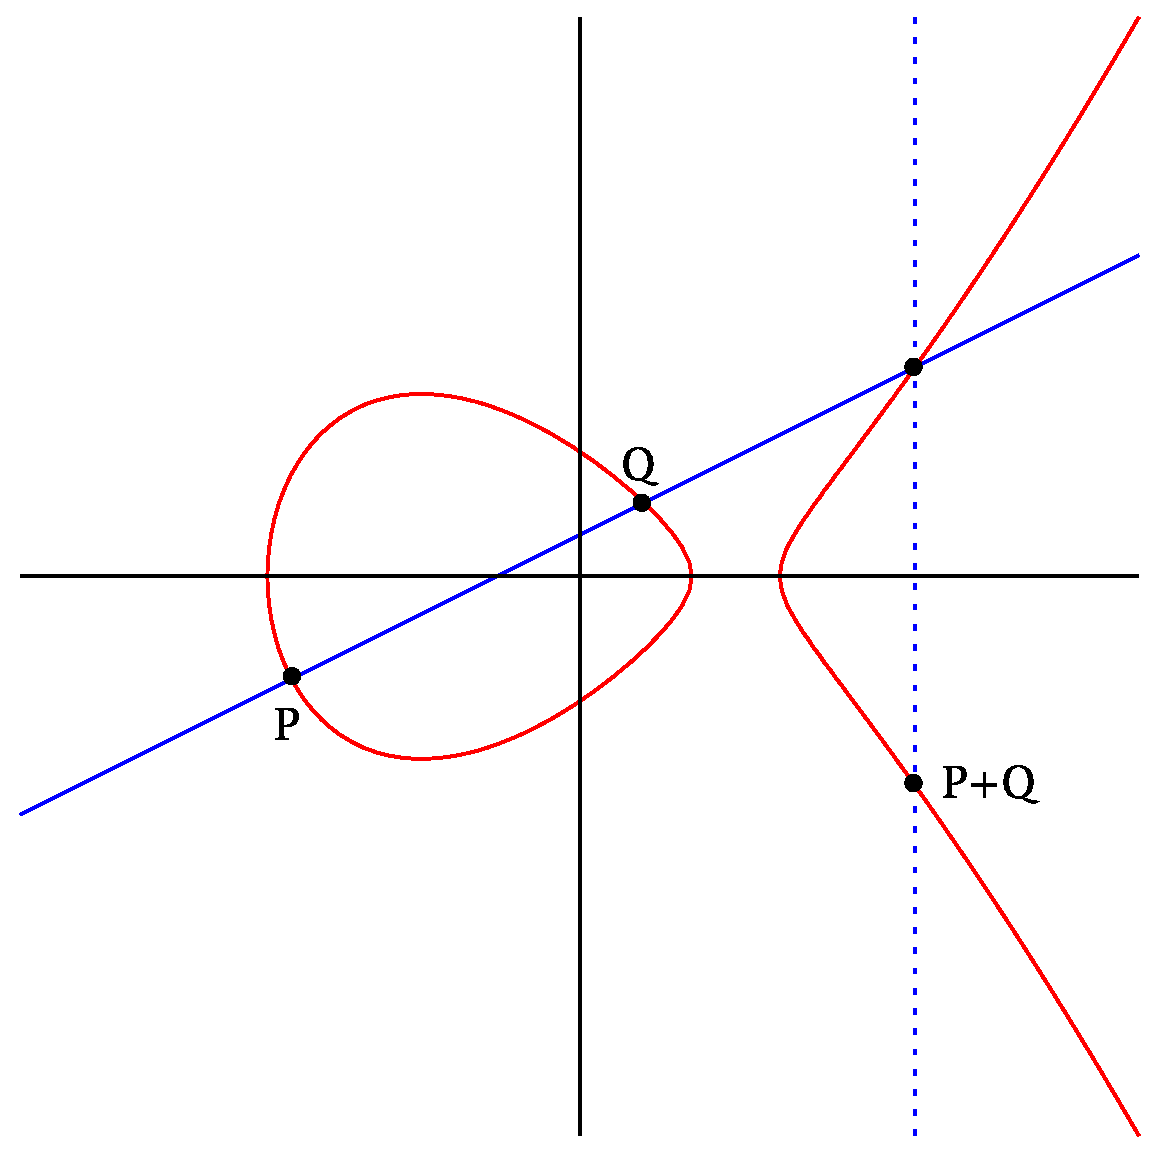
\includegraphics[width=0.5\textwidth]{isogeny/ec-add}
  \caption{Chord-tangent law on an elliptic curve defined over the reals.}
  \label{fig:chord-tangent}
\end{figure}

The definition is pictured in Figure~\ref{fig:chord-tangent}. For a
proof that this defines indeed a group law on the points of $E$, with
$\0$ being the identity element, see \cite[II, $\S2$]{silverman:elliptic}.

\begin{definition}[Rational points]%
  \nomenclature[E]{$E(\K)$}{Set of $\K$-rational points of an elliptic curve $E$}
  Let $E$ be an elliptic curve defined over $\K$, the set of
  \emph{$\K$-rational points}\index{rational~point} $E(\K)$ is 
  \begin{equation}
    \label{eq:119}
    E(\K) = E \cap \Proj^2(\K)
    \text{.}
  \end{equation}
\end{definition}

If $P$ and $Q$ are rational points, the lines $L$ and $L'$ are defined
by equations over $\K$, thus $E(\K)$ forms a subgroup of $E$. To allow
calculations in $E(\K)$ without having to lift the coefficients in an
algebraic closure, it is convenient to give explicit formulas for the
chord-tangent law. 

We shall give the formulas for affine coordinates. From now on, if $P$
is an affine point of $E$, we denote by $x(P)$ its abscissa and by
$y(P)$ its ordinate.

\begin{proposition}
  Let $E$ be the elliptic curve defined by Eq.~\eqref{eq:112}. Let
  $P$, be a point of $E$ different from $\0$, the coordinates of $-P$
  are given by
  \begin{equation}
    \label{eq:120}
    x(-P) = x(P)\text{,}\qquad y(-P)=-y(P) -a_1x(P) - a_3
    \text{.}
  \end{equation}
  Let $P,Q$ be points of $E$ different from $\0$ and let $Q\ne-P$, the
  coordinates of $P+Q$ are given by
  \begin{equation}
    \label{eq:121}
    \begin{aligned}
      \lambda &= \begin{cases}
        \frac{y(Q) - y(P)}{x(Q) -x(P)} &\text{if $P\ne Q$,}\\
        \frac{3x(P)^2+2a_2x(P)+a_4-a_1y(P)}{2y(P)+a_1x(P)+a_3} &\text{if $P=Q$,}
      \end{cases}\\
      x(P+Q) &= \lambda^2+a_1\lambda-a_2-x(P)-x(Q)\text{,}\\
      y(P+Q) &= -(\lambda+a_1)x(P+Q) - y(P) + \lambda x(P)-a_3\text{.}
    \end{aligned}
  \end{equation}
\end{proposition}

\begin{definition}[Kummer surface]
  The \index{Kummer~surface}\emph{Kummer surface} of an elliptic curve
  $E$, denoted by $K_E$\nomenclature[KE]{$K_E$}{Kummer surface of an
    elliptic curve}, is the quotient of $E$ by the equivalence
  relation $P\simeq-P$.
\end{definition}

\begin{remark}
  The Kummer surface can be represented by taking the abscissas of the
  points of $E$. It is not anymore a group, but we can still compute
  scalar multiples of its points. In fact, from the addition formulas
  we deduce for $P\ne-P$
  \begin{equation}
    \label{eq:128}
    x([2]P) = \frac{x^4-b_4x^2-2b_6x-b_8}{4x^3+b_2x^2+2b_4x+b_6}
    \text{,}
  \end{equation}
  where $x=x(P)$; and for $P\ne Q$
  \begin{equation}
    \label{eq:129}
    x(P+Q) + x(P-Q) =
    \frac{2\pi\sigma + b_2\pi + b_4\sigma + b_6}{(x(P)-x(Q))^2}
    \text{,}
  \end{equation}
  where $\pi=x(P)x(Q)$ and $\sigma=x(P)+x(Q)$. 

  Then, to compute $x([n]P)$, we start from $x(P)$ and $x([2]P)$, and
  we iteratively apply
  \begin{equation}
    \label{eq:130}
    \begin{aligned}[]
      [2i]P   &= [2][i]P\text{,}\\
      [2i+1]P &= [i+1]P + [i]P\text{,}
    \end{aligned}
  \end{equation}  
  or
  \begin{equation}
    \label{eq:131}
    \begin{aligned}[]
      [2i+1]P &= [i+1]P + [i]P\text{,}\\
      [2i+2]P &= [2][i+1]P\text{,}
    \end{aligned}
  \end{equation}
  until we reach $[n]P$.
\end{remark}

For $n\in\Z$, we denote by $[n]P$ the point%
\nomenclature[nP]{$[n]P$}{Scalar multiple of a point of an elliptic
  curve} $\overbrace{P+P+\cdots+P}^{n\text{ times}}$ if $n>0$, or the
point $[-n](-P)$ if $n<0$, or $\0$ if $n=0$. The map
\begin{equation}
  \label{eq:122}
  \begin{aligned}[]
    [n]_E : E(\K) &\ra E(\K)\text{,}\\
    P &\mapsto [n]P
  \end{aligned}
\end{equation}
is a group endomorphisms of $E(\K)$. 

\begin{definition}
  The $n$-th \emph{torsion subgroup} of $E$ is
  \begin{equation}
    \label{eq:123}
    E[n] = \{P\in E(\K) \,|\, [n]P=\0\}
    \text{,}
  \end{equation}
  its points are called%
  \nomenclature[E]{$E[n]$}{$n$-torsion subgroup of an elliptic curve
    $E$}
  \index{elliptic~curve!torsion~subgroup}\index{torsion~point}\emph{$n$-torsion
    points}.
\end{definition}

Since addition is an algebraic map, multiplication by $n$ is algebraic
too. It can be shown that there exist polynomials
$\psi_n,\theta_n,\omega_n\in\K(E)$ such that
\begin{equation}
  \label{eq:124}
  [n](x,y) = \left(\frac{\theta_n(x,y)}{\psi_n(x,y)^2},
    \frac{\omega_n(x,y)}{\psi_n(x,y)^3}\right)
  \text{.}
\end{equation}

\begin{definition}[Division polynomials]
  The polynomial $\psi_n$ is called the
  \index{division~polynomial}\emph{$n$-th division polynomial}.
\end{definition}

\begin{remark}
  The division polynomials can be computed from the addition formulas
  via a double-and-add approach. Their importance comes from the fact
  that $\psi_n$ vanishes on $E[n]$.
\end{remark}

From the formulas for the division polynomials one can deduce the
structure of the $n$-torsion.

\begin{theorem}
  Let $p$ be the characteristic of $\K$. If $p$ does not divide $n$
  \begin{equation}
    \label{eq:126}
    E[n] \isom \Z/n\Z\times\Z/n\Z
    \text{;}
  \end{equation}
  if $p\ne0$, then for every $i>0$ either
  \begin{equation}
    \label{eq:127}
    E[p^i] = \{\0\}\text{,} 
    \qquad\text{or}\qquad E[p^i] \isom \Z/p^i\Z
    \text{.}
  \end{equation}
\end{theorem}

\begin{definition}[Supersingular, ordinary]
  An elliptic curve $E$ is said to be
  \index{elliptic~curve!supersingular}\index{supersingular}\emph{supersingular}
  if $E[p^i]=\{\0\}$ for any $i$; it is said to be
  \index{elliptic~curve!ordinary}\emph{ordinary} otherwise.
\end{definition}

\begin{definition}[Tate module]
  Let $\ell$ be a prime, the \index{Tate~module}\emph{$\ell$-adic Tate
    module}
  $\mathcal{T}_\ell(E)$\nomenclature[Tl]{$\mathcal{T}_\ell(E)$}{$\ell$-adic
    Tate module} is the group
  \begin{equation}
    \label{eq:132}
    \mathcal{T}_\ell(E) = \varprojlim_n E[\ell^n]
  \end{equation}
  with respect to the projections
  \begin{equation}
    \label{eq:133}
    [\ell]_E : E[\ell^{n+1}] \ra E[\ell^{n}]
    \text{.}
  \end{equation}
\end{definition}

\begin{proposition}
  The Tate module has a natural structure of
  $\Z_\ell$-module\nomenclature[Zp]{$\Z_p$}{$p$-adic
    integers\nomnorefpage}. As such
  \begin{equation}
    \label{eq:134}
    \mathcal{T}_\ell(E) \isom
    \begin{cases}
      \Z_\ell\times\Z_\ell &\text{if $\ell\ne p$,}\\
      \Z_p &\text{if $\ell=\car(\K)$ and $E$ is ordinary,}\\
      \{\0\} &\text{if $E$ is supersingular.}
    \end{cases}
  \end{equation}
\end{proposition}


\subsection{Isomorphisms}
\label{sec:isomorphisms}

Concerning the uniqueness of the representation by a Weierstrass
equation, we have that the only changes of variables that preserve the
point at infinity  are
\begin{equation}
  \label{eq:116}
  \begin{aligned}
    x &= u^2x' + r\text{,}\\
    y &= u^3 + u^2sx' + t\text{,}
  \end{aligned}
\end{equation}
with $r,s,t,u\in\clot{\K}$.

\paragraph{Simplified forms} If $p>3$ it is well known that the curve
$E$ is isomorphic to a curve in the form
\begin{equation}
  \label{eq:weierstrass>3}
  y^2 = x^3 + ax + b
\end{equation}
and its $j$-invariant is $j(E) = \frac{1728(4a)^3}{16(4a^3 + 27b^2)}$.

When $p=3$, since $E$ is ordinary, it is isomorphic to a curve
\begin{equation}
  \label{eq:weierstrass=3}
  y^2 = x^3 + ax^2 + b
\end{equation}
and its $j$-invariant is $j(E) = -\frac{a^3}{b}$.

Finally, when $p=2$, since $E$ is ordinary, it is isomorphic to a curve
\begin{equation}
  \label{eq:weierstrass=2}
  y^2 + xy = x^3 + ax^2 + b
\end{equation}
and its $j$-invariant is $j(E) = \frac{1}{b}$.

These isomorphism are easy to compute and we will always assume that
the elliptic curves given to our algorithms are in such simplified
forms.

\subsection{Isogenies}
\label{sec:isogenies}

Elliptic curves are endowed with the classic group structure through
the chord-tangent law. A group morphism having finite kernel is called
an \emph{isogeny}. Isogenies are regular maps, as such they can be
represented by rational functions. An isogeny is said to be
$\K$-rational if it is $\K$-rational as regular map; its degree is the
degree of the regular map.

One important property about isogenies is that they factor the
multiplication-by-$m$ map.

\begin{definition}[Dual isogeny]
  Let $\I : E \rightarrow E'$ be a degree $m$ isogeny. There exists an
  unique isogeny $\hat{\I} : E' \rightarrow E$, called the \emph{dual
    isogeny} such that
  \[\I\circ\hat{\I} = [m]_E \qquad\text{and}\qquad \hat{\I}\circ\I =
  [m]_{E'}\]
\end{definition}

As regular maps, isogenies can be separable, inseparable or purely
inseparable. In the case of finite fields, purely inseparable
isogenies are easily understood as powers of the frobenius map. Let
\[E^{(p)} : y^2 + a_1^pxy + a_3^py = x^3 + a_2^px^2 + a_4^px + a_6^p\]
then the map
\begin{align*}
  \frobisog : E &\rightarrow E^{(p)}\\
          (x,y) &\mapsto (x^p,y^p)
\end{align*}
is a degree $p$ purely inseparable isogeny. Any purely inseparable
isogeny is a composition of such frobenius isogenies.

Let $E$ and $E'$ be two elliptic curves defined over $\F_q$, by
finding an \emph{explicit isogeny} we mean to find an
($\F_q$-rational) rational function from $E(\clot{\F}_q)$ to
$E'(\clot{\F}_q)$ such that the map it defines is an isogeny.

\begin{figure}
  \centering
  \[\xymatrix{
    E \ar[r]^{[m]}\ar@/_1pc/[rrr]_{\I'} & E \ar[r]^\I & E' \ar[r]^{\frobisog^n} & E'^{(p^n)}\\
  }\]
  \label{fig:fact}
  \caption{Factorization of an isogeny. $\I'$ has kernel $E[m]\oplus\ker\I$.}
\end{figure}

Since an isogeny can be uniquely factored in the product of a
separable and a purely inseparable isogeny, we focus ourselves on the
problem of computing explicit separable isogenies. Furthermore one can
factor out multiplication-by-$m$ maps, thus reducing the problem to
compute explicit separable isogenies with cyclic kernel (see figure
\ref{fig:fact}).

In the rest of this paper, unless otherwise stated, by $\ell$-isogeny
we mean a separable isogeny with kernel isomorphic to $\Z/\ell\Z$.

\paragraph{Vélu formulae}
For any finite subgroup $G \subset E(\clot{\K})$, Vélu formulae
\cite{Vel71} give in a canonical way an elliptic curve $\bar{E}$ and
an explicit isogeny $\I:E\rightarrow \bar{E}$ such that
$\ker\I=G$. The isogeny is $\K$-rational if and only if the polynomial
vanishing on the abscissae of $G$ belongs to $\K[X]$.

In practice, if $E$ is defined over $\F_q$ and if
\[h(X) = \prod_{\substack{P\in G\\P\ne\0}}(X - x(P)) \in \F_q[X]\]
is known, Vélu formulae compute a rational function
\begin{equation}
  \label{eq:isog}
  \bar{\I}(x,y) = \left(\frac{g(x)}{h(x)}, \frac{k(x,y)}{l(x)}\right)  
\end{equation}
and a curve $\bar{E}$ such that $\bar{\I} : E\rightarrow\bar{E}$ is an
$\F_q$-rational isogeny of kernel $G$. A consequence of Vélu formulae
is
\begin{equation}
  \label{eq:velu-deg}
  \deg g = \deg h + 1 = \card{G}
  \text{.}
\end{equation}

Given two curves $E$ and $E'$, Vélu formulae reduce the problem of
finding an explicit isogeny between $E$ and $E'$ to that of finding
the kernel of an isogeny between them. Once the polynomial $h(X)$
vanishing on $\ker\I$ is found, the explicit isogeny is computed
composing Vélu formulae with the isomorphism between $\bar{E}$ and
$E'$ as in figure \ref{fig:velu}.

\begin{figure}
  \centering
  \[\xymatrix{
    E \ar[r]^{\bar{\I}} \ar[rd]^\I & \bar{E} \ar[d]^{\simeq}\\
    & E'
  }\]
  \caption{Using Vélu formulae to compute an explicit isogeny.}
  \label{fig:velu}
\end{figure}



over C: periods, weierstrass series

over finite field: number of points? frobenius


% Local Variables:
% mode:flyspell
% ispell-local-dictionary:"american"
% mode:TeX-PDF
% mode:reftex
% TeX-master: "../these"
% End:
%
% LocalWords:  Schreier Artin pseudotrace frobenius bivariate Joux Sirvent FFT
% LocalWords:  Couveignes isogenies Schoof isogeny cryptosystems Lercier
% LocalWords:  precomputation arithmetics polylogarithmic Karatsuba
% LocalWords:  endomorphisms
